% -*- TeX-master: "Qualificacao.tex" -*-
%!TEX root = Qualificacao.tex
\chapter{Reinforcement Learning}\label{cap:RL}
\vspace{-1cm}

% Frase citação inicial {{{1
% \begin{flushright}
% \begin{minipage}{0.7\linewidth}
%     \emph{``\dots''}
% \end{minipage}
% \end{flushright}
%
% \begin{flushright}
% Cicrano
% \end{flushright}
%
%\vspace{1cm}

% Intro CAP {{{1
The main aim of control systems is to modify the behavior of a dynamical system in such a way that the final system achieves some predetermined performance, such as tracking a trajectory or keeping a fixed value, despite eventual disturbances on the system. 
Many approaches have been developed along the last two 
% \todo[color=orange]{\textbf{LAA: }  cite um dos livros ``clássicos de controle''.} Citei Ogata
centuries \citep{ogata2010}. 
One of these approaches solves the problem of assigning a numerical performance index to each state trajectory of the system and then finding a control sequence, or a control policy that drives the system along the trajectory with the best index. This methodology is known in the control literature as Optimal Control, with early works in 1940s by Pontryagin and Bellman \citep{bellmann1957}.\todo{referencia.}  

In particular, the Dynamic Programming (DP, for short) introduced by Bellman deals with this kind of problem for discrete time dynamic systems generating a sequence of states under the influence of control and using a concept that became know as Bellman's Principle to find in a iterative fashion, the optimum solution\todo{reference.}. 

Among 
% \todo[color=orange]{\textbf{LAA: } longo (parágrafo?)}
the advantages of the DP, is its ability to deal with linear and nonlinear, time variant or time invariant systems,  and to cope with restrictions on state or control spaces. This makes DP an attractive methodology do be used on nowadays control problems.

But the initial approach find problems when the number of possible states or control actions are too large. 
For such systems, the computational effort could become impracticable.
Another problem is that a model needs to be previously known.

The idea of finding a solution in the absence of a model has been explored since 
\todo{referências}
the 1960s.
Since then many approaches have been presented to design controllers without a dynamic model. 
\todo{referencias a metodos DDC}
% Reinforcement Learning (RL for short) is one of \todo[color=orange]{\textbf{LAA: } \textit{such} é melhor que \textit{these} pq não mencionou nenhum ainda.} such methods.
Arising from DP, RL aims to solve the optimization control problem without the need of a model and using functions approximations to deal with large-order systems.
In the 80s the interest grew and led to the development of the field of RL. 
\todo{colocar aqui referências para Werbos, Watkins, etc...}

% The central theme of RL is the design of algorithms that learn control policies solely from the knowledge of transition samples trajectories, which are collected beforehand or by online interaction with the system. \todo{melhorar}
The central theme of RL is the development of strategies to learn control policies from the knowledge only of transition samples or trajectories, which could be collected from the system in a batch or a recursive way. 

% - one approach to modify behavior of dynamical systems to achieve predetermined aims is to assign a numerical performance index to each state trajectory of the system and then find the control Policy that drives the system along the trajectory with the best index.

% - Optimal control has early works on 1940s with Pontryagin and Bellman.
% - Dynamic programming: introduced by Bellman; \todo{find a reference.}

% Our focus is on reinforcement learning methods that learn while interacting with the environment \cite{sutton2011}
% \cite{busoniu2017} lists the next Three classes o
Three major approaches can be listed in the RL field for control: methods based on use of tabular value functions for policy evaluation and improvement; methods based on use of value function approximations to deal with policy evaluation and improvement in continuous state-spaces; and methods that use function approximation to search direct for policy improvement, without the need of value functions.  

This chapter gives an introduction in the three class of methods listed above.
% In fact, these three classes of techniques developed initially for DP to deal with optimization problems where a model is available were then extended to work in a model-free fashion, resulting in some fundamental methods for RL.
Section \ref{sec:description} gives some basic definitions. In sequence, section \ref{sec:DP} introduce some basic concepts of dynamic programing, since RL methods based on value functions estimations arises from dynamic programming. The methods introduced in section \ref{sec:DP} are adapted to the case where no model of the environment are available, resulting in RL methods based on tabular value-functions predictions, for prediction and control problems. The last section, \ref{sec:funcApprox}, presents some approaches to use function approximations to deal with RL problems involving problems with huge  or infinite number of states, like the continuous state-space case.  Sections \ref{sec:valFunApp} to \ref{sec:offPoliceControlFA} deals with value-functions approximations, and at the end, in section \ref{sec:PGM}, a different approach of policy improvement methods, using function approximations direct for policy approximation, known as policy gradient methods, are presented.

% extend the methods to cases where tabular value functions aren't enough, like problems involving continuous states, using the concept of function approximations. At the end a
% , with the intention use it as tools to solve data-driven control problems~\todo{mudar todo o parágrafo (vide 1a revisão do Aguirre). A ideia é falar um pouco do que será tratado em cada seção (talvez) do capítulo. Porém acho melhor fazer isso quando ficar tudo pronto.}.

%}}}

\section{Description of the problem} 
\label{sec:description}
% \todo{Colocar conceito de estado? Sinal de controle? Environment}
% \todo[color=orange]{\textbf{LAA: } Sim. Coloque as equações de estado e defina as variáveis.}

\begin{description}
    % \item[Requirement:] availability of a signal that completely describes the process.
    % \item[The environment:] \todo{Olhar no \cite{sutton2011} ou nos slides do David Silver o conceito}
    % \item[The control:]
    \item[The process:] 
      Commonly know in RL field as the \emph{environment},  is the physical body of de decision-making entity, everything outside the main controller,  the sensors and actuators as any fixed lower level controllers, are all considered to be a part of the process \citep{busoniu2017}. 
      In control community, is common to represent the process as the following state equation:
      \begin{equation}
          \vx_{k+1} = \vf_k(\vx_k,\vu_k), \qquad k = 0, 1, \dots, N-1
      \label{eq:dss},
      \end{equation}
      where $k$ is the stage, or time, index; $\vx_k \in \R^n$ is the \emph{state} of the system, that belongs to some set $\Omega_k$, where $n$ is the number of state variables; $\vu_k \in \R^p$ is the control signal to be selected from some set $\mathcal{U}_k(\vx_k)$, where $p$ is the number or control signals (or actions); $N$ is the horizon, or the number of stages the control is applied. Can be a finite value for a \emph{finite-step} system trajectory (known as \emph{episodic task} ou simple \emph{episode} in RL field), or tends to infinity for \emph{infinity-step} system trajectory (or \emph{continuing tassk} in RL).
      \todo{Mencionar a formulacao do processo em termos de MPD.} 

      Figure \ref{fig:stages} illustrates the time evolution of the states, according to \eqref{eq:dss} for a finite-step trajectory.

      \begin{figure}[htpb]
          \centering
          % \includegraphics[width=0.8\textwidth]{}
              \begin{tikzpicture}[->,>=stealth',shorten >=1pt,auto,node distance=2.5cm, thick]
      \tikzstyle{every state}=[draw=black,fill=blue!20,text=black]
      \tikzstyle{dots}=[thick,draw=none,fill=none,text=black]
      \tikzstyle{place}=[draw=none,fill=none,text=black!75]
      \tikzstyle{texto}=[draw=none,fill=none,text=black]
      \node[state] (A)              {$x_0$};
      \node[dots ] (B) [right of=A] {$\cdots$};
      \node[state,draw=blue!75] (C) [right of=B] {$x_{k}$};
      \node[state,draw=blue!75] (D) [right of=C,xshift=1cm] {$x_{k+1}$};
      \node[dots ] (E) [right of=D] {$\cdots$};
      \node[state] (F) [right of=E] {$x_N$};
      \node[place] (k) [below of=C, yshift=1.5cm] {$|$};
      \node[place] (l) [below of=D, yshift=1.5cm] {$|$};
      \node[texto] (f) [above of=F, yshift=-1.5cm] {Terminal Cost $r_N$};
      \node[texto,text=black!75] (t1) [below of=C, yshift=1cm, xshift=1.75cm] {Stage $k$};
      \node[texto] (t2) [below of=C, yshift=2.2cm, xshift=1.75cm, text=blue] {Control $u_k$};

      \path (A) edge node {} (B)
            (B) edge node {} (C)
            (C) edge [draw=blue!75,ultra thick] node [text=blue] {Cost $r_k$} (D)
            (D) edge node {} (E)
            (E) edge node {} (F);
      % \path (C) [draw=blue] edge node {} (D);
      \draw [dashed,<->,draw=black!75] (k) -- (l);
    \end{tikzpicture}

          \caption{Deterministic N-stage episodic task.}
          \label{fig:stages}
      \end{figure} 
      \todo{Falar mais da figura..}

    \item[The controller:] Frequently called \emph{agent}  in RL field, is the decision maker, interacts with the process using an \textit{control signal} (known as  \emph{action signal}, or simple \emph{action}, in RL field), aiming to influence the process. To generate this action signal, the controller uses the knowledge of the current \textit{state signal} that describes the state of processes and the \textit{reward signal}, a scalar signal which quantifies the current performance of the process.

    \item[The Policy:] A mapping from states $\vx_k$ into actions (what action should be taken in each state).
      \todo{terminar}
      \begin{equation}
          \vu_k = \vpi(\vx_k) \quad \text{for } k=1,\ 2,\ 3,\ ...,\ N
      \label{eq:policy}.
      \end{equation}

    \item[The Stage Cost or Reward:] The stage cost 
      % \todo{confirmar aqui se $r_k$ ou $r_{k+1}$}
      $r_{k}$ is a result of the transition from state $\vx_k$ to $\vx_{k+1}$ when the action  $\vu_k$  is taken.  
      % \todo{falar aqui da questão das ``rewards ou penalties''}
      It is a measure that quantifies some criteria. The stage cost depends on the state-action trajectory and, consequently depends in the adopted policy, as stated in \eqref{eq:policy}.
      In control applications, where it is usual to minimize the total cost,  the term \emph{stage cost} is adopted. In computer science, where it is usual to maximize the total cost, the therm  \textit{reward} is usually adopted.
      Here, as we will deal with control problems the term \textit{stage cost} will be used instead.

      Figure \ref{fig:stages} illustrates the concept of a stage cost. In stage $k$, when a control $u_k$ is taken, taking the trajectory from the state $k$ to  $k+1$, a cost of $r_k$ is spent.

    \item[The Cost-to-go or Return:] The cost, or cost-to-go, is the cumulative stage costs over the trajectory performed given a fixed policy 
      % \todo{is the cumulative reward over the course of interaction}
      . It is a function of the initial state $\vx_0$, and the control actions sequence $\left\{ \vu_0, \dots, \vu_{N-1}\right\}$.
      For deterministic episodic tasks, it can be represented by 
      \begin{equation}
          R(\vx_0;\vu_0, \dots, \vu_{N-1}) = r_1+r_2+\dots+r_N = \sum_{k=1}^N{ r_k(\vx_k, \vu_k) } 
      \label{eq:return}.
      \end{equation}
      % \todo[color=cyan]{Por algum motivo o latex nao estah colocando espaco depois das virgulas nas equacoes (posso forcar isso com uma barra invert., mas nao seria a melhor solucao). Vou olhar isso depois.}
      For infinite tasks, when the trajectories can be infinitely long, it is common to consider a discounted cost \todo{na equacao \ref{eq:discReturn}, nao seria $J(\vx_0;\vu_0, \dots, \vu_{N-1})$? Olhar isso.} as

      \begin{equation}
        R(\vx_0) = \lim_{N\to\infty}\sum_{k=1}^N \gamma^{k-1} r_k(\vx_k,\vu_k)
      \label{eq:discReturn},
      \end{equation}

      %\todo{Confirmar em \eqref{eq:discReturn} e \eqref{eq:return} se usar mesmo $k$ ou outra variavel} where $0 < \gamma \le 1$ is called \textit{discount factor} and weights the stage costs in a  exponentially time decreasing way, giving more importance to early stage costs than the last ones. For simplicity, in this section the total cost will be expressed as \eqref{eq:discReturn} with the $\lim_{N\to \infty}$ omitted. So, $N$ should be taken as finite for episodic tasks or infinity for endless tasks and $\gamma$ should be taken as $\gamma =1$ for undiscounted tasks and $\gamma < 1$ one for the discounted ones.
      For problems with stochastic transitions, as will be seen later, in section \eqref{sec:SDP}, the total cost is taken as the expectation of \eqref{eq:discReturn}.
      In control engineering the term total cost, ou simply cost is commonly adopted, while in computer science the term \textit{Return} is usual.

    \item[The cost function] The cost function $J(x_0,u_0)$ here is defined as the expected value of the cost-to-go, i.e. the expected value to follow an arbitrary policy, so
      \begin{equation}
        J(\vx_0;\vu_0, \dots, \vu_{N-1}) = \E\left\{ R(\vx_0;\vu_0, \dots, \vu_{N-1}) \right\}
      \label{eq:cost_fun_return}.
      \end{equation}
      In RL literature is common to refer to the cost function as \textit{state value function}. Here, the author chooses to use the term \textit{cost function } due to be more usual in control applications.
      Note that for a deterministic case, the cost function is equal to the return.

    \item[The Goal:] In DP or RL the challenge is to find the optimal policy $\pi^*(\vx_k)$ that maximizes (or minimizes) the return~\eqref{eq:return} or~\eqref{eq:discReturn}, i.e.\ the long term performance, using only the reward information that describes the imediate performance for every initial condition.
      For that, the availability of a signal that completely describes the process is required. 
      % \todo{é requerida também a função de custo?}
      % \begin{equation}
      %     \pi^*(\vx_0) \in \argma\vx_{u} \sum_{k=1}^N{ r_k }
      % \label{eq:optPolicy}.
      % \end{equation}
      % If transitions are stochastic the aim is to maximize (or minimize) the expectation of \eqref{eq:return} or \eqref{eq:discReturn}.
      % \todo{mudar isso para ``returns''?}
  \end{description}


\section{Dynamic Programming} 
\label{sec:DP}

Reinforcement Learning, \todo{já falei isso anteriormente!} or RL for short, is intrinsically related with Dynamic Programming, since the method can be seen as an extension of  Dynamic Programming \todo{já falei isso anteriormente!}(DP), that learns a suboptimal control policy, online or offline, without the need of a model of the environment. \todo{Ref. aqui} 
For that reason this section gives a brief introduction to DP.
\todo{Colocar algo sucinto aqui sobre a origem da Programação dinâmica?}

In the most general case the problem formulation involves random variables, e.g. the control policy could be random, resulting in a random state transition. But, for the sake of simplicity, we will start with the deterministic case and then, when some fundamental concepts is given, the stochastic approach will be presented. 

Many DP problems can be represented by a finite steps trajectory or, as known in RL terminology, as an episodic task. In this kind of problem, the task (or trajectory) always ends at some state. In another kind of problems, the task never ends, resulting in a infinite-step trajectory. In RL, this last case is known as the continuing case. The episodic case is conceptually simpler than the continuing one. For this reason generally, in this text, the concepts will be presented in episodic context first and then, extended to the continuing case. 

\subsection{Deterministic Dynamic Programming}

Consider the discrete-time state space representation of a dynamic system presented in \eqref{eq:dss}. 
% the form \todo[color=orange]{\textbf{LAA: } Defina as dimensões.}
% \begin{equation}
    % \vx_{k+1} = \vf_k(\vx_k,\vu_k), \qquad k = 0, 1, \dots, N-1
% \label{eq:dss},
% \end{equation}
% where $k$ is the stage, or time, index; $\vx_k \in \R^n$ is the state of the system; $\vu_k$ is the control signal or decision variable or action, to be selected from some set $\mathcal{U}_k(\vx_k)$; \todo{Colocar conceitos do conj. $\mathcal{U}$ (controles admissíveis) e $\Omega$.} $\vf_k$ is a function of $(\vx_k,\vu_k)$ that represents the transition from $\vx_k$ to $\vx_{k+1}$, when $\vu_k$ is applied; $N$ is the horizon or number of times the control is applied.
% \begin{description}
%     \item[$k$] is the time index,
%     \item[$\vx_k$] is the state of the system,
%     \item[$\vu_k$] is the control signal or decision variable or action, to be selected from some set $\mathcal{U}_k(\vx_k)$, \todo{Colocar conceitos do conj. $\mathcal{U}$ (controles admissíveis) e $\Omega$.}
%     \item[$\vf_k$] is a function of $(\vx_k,\vu_k)$ that represents the transition from $\vx_k$ to $\vx_{k+1}$, when $\vu_k$ is applied,
%     \item[$N$] is the horizon or number of times the control is applied.
% \end{description}
The main objective in DP is to find a control policy that minimizes a cost function as stated in \eqref{eq:discReturn}.
This can be accomplished using the \textit{principle of optimality} that states the following 
\begin{teo}{Principle of Optimality \citep{bertsekas2019}
\\} \label{teo:bellmanopt}
% \todo{dar uma olhada na definição do Kirk.}
% \todo[color=cyan]{coloquei na íntegra o princípio de otimalidade de Bellman aqui, mas não estou gostando muito do jeito que ele coloca. Vou tentar melhorar.}
    Let $u^*_0, \dots, u^*_{N-1}$ be an optimal control sequence, which together with $\vx_0$ determines the corresponding state sequence $\vx_1^*, \dots, \vx_N^*$ via the system equation \eqref{eq:dss}. Consider the subproblem whereby we start at $\vx_k^*$ at time $k$ and wish to minimize the  ``cost-to-go'' from time $k$ to time  $N$,
     \begin{equation}
       J(\vx,\vu) = r_k(\vx_k^*,\vu_k) + \sum_{m=k+1}^{N-1} r_m(\vx_m,\vu_m) + r_N(\vx_N)
    \label{eq:optPrin},
    \end{equation}
  % \todo[color=orange, size=\tiny]{\textbf{LAA: } onde está o = desta equação?} \todo[color=cyan, size=\tiny]{\textbf{To LAA: } \textbf{Resposta:} Vou mudar todo o teorema ainda. Coloquei assim pois como havia dito, coloquei na íntegra como apresentado por \cite{bertsekas2019}, e ele apresenta assim. Tb achei estranho.  }
    over $\vu_k, \dots, \vu_{N-1}$ with $\vu_m \in \mathcal{U}_m$, $m=k,\dots,N-1$. Then the truncated optimal control sequence  $u^*_k, \dots, u^*_{N-1}$ is optimal for this subproblem.
\end{teo}
As stated in \cite{bertsekas2019}, the optimality principle can be summarized as: ``\textit{the tail of an optimal sequence is optimal for the tail subproblem}''. Figure
\todo{Terminar a figura~\ref{fig:BellmanTail}: colocar $r_k's$, corrigir tamanho dos círculos. Contextualizá-la melhor também.}
~\ref{fig:BellmanTail} illustrates the concept.
\begin{figure}[htpb]
    \centering
    % \missingfigure{Figura Bellman aqui}
        \begin{tikzpicture}[->,>=stealth',shorten >=1pt,below,node distance=2.3cm, thick]
      \tikzstyle{every state}=[draw=black,fill=blue!20,text=black]
      \tikzstyle{dots}=[thick,draw=none,fill=none,text=black]
      \tikzstyle{place}=[draw=none,fill=none]
      \tikzstyle{texto}=[draw=none,fill=none,text=black]
      \node[state] (A)              {$x_0$};
      \node[state] (B) [right of=A] {$x_{1}$};
      \node[dots ] (C) [right of=B] {$\dots$};
      \node[state] (D) [right of=C] {$x^*_{k}$};
      \node[dots ] (E) [right of=D] {$\dots$};
      \node[state] (F) [right of=E] {$x^*_{N-1}$};
      \node[state] (G) [right of=F] {$x^*_N$};
      \node[place] (k) [below of=A, yshift=1cm] {$|$};
      \node[place] (l) [below of=G, yshift=1cm] {$|$};
      \node[place] (m) [above of=D, yshift=-1.4cm, text=red] {$|$};
      \node[place] (n) [above of=G, yshift=-1.4cm, text=red] {$|$};
      \node[texto] (f) [below of=G, yshift=2cm, xshift=0.75cm, text=blue] {$r_N$};
      \node[texto,text=black] (t1) [below of=D, yshift=0.7cm] {Optimal control sequence};
      \node[texto,text=red] (t1) [above of=E, yshift=-1.1cm, xshift=1.25cm] {Tail subproblem};
      % \node[texto] (t2) [below of=C, yshift=2.2cm, xshift=1.25cm, text=blue] {$r_k$};

      \path (A) edge node [text=black] {$u^*_0$} (B) 
            (B) edge node [text=black] {$u^*_1$} (C)
            (C) edge node [text=black] {$u^*_{k-1}$} (D)
            (D) edge node [text=red] {$u^*_k$} (E)
            (E) edge node [text=red] {$u^*_{N-2}$} (F)
            (F) edge node [text=red] {$u^*_{N-1}$} (G);
      % \path (C) [draw=blue] edge node {} (D);
      \draw [dashed,<->,draw=black!75] (k) -- (l);
      \draw [dashed,->,draw=red] (m) -- (n);
    \end{tikzpicture}

    \caption{Illustration of the Bellman's principle of optimality }%\[FONT:  Adapted from \cite{bertsekasReinforcementLearningOptimal2019}).}
    \label{fig:BellmanTail}
\end{figure}
According to \eqref{eq:discReturn}, a cost function that describes a requirement to be optimized, starting from time $k$, can be rewritten as 
\begin{equation}
    J(\vx_k;\vu_k, \cdots, \vu_{N-1}) = \sum_{m=k}^{N-1} r_m(\vx_m,\vu_m) + r_N(\vx_N)
\label{eq:costFunctiok},
\end{equation}
where $r_N(\vx_N)$ is the terminal cost at the final stage, i.e. the terminal cost.

Once the goal is to find the control sequence $\vu_k, \vu_{k+1}, \dots, \vu_N$, that minimizes the cost-to-go function \eqref{eq:costFunctiok}, this can be accomplished computing
\begin{equation}
    J^*_k(\vx_k) = \min_{\vu_m \in \mathcal{U}_m} J(\vx_k;\vu_k, \cdots, \vu_{N-1}), \qquad \text{for } m=k, \dots, N-1
\label{eq:optCostFun1}.
\end{equation}
Substituting \eqref{eq:costFunctiok} in \eqref{eq:optCostFun1} and rewriting as
\begin{align}
    J^*_k(\vx_k) &= \min_{\vu_m \in \mathcal{U}_m} \left[ \sum_{m=k}^{N-1} r_m(\vx_m,\vu_m) + r_N(\vx_N) \right] \nonumber\\
             &= \min_{\vu_k \in \mathcal{U}_k} \left[ r_k(\vx_k, \vu_k) +\min_{\vu_m \in \mathcal{U}_m} \left[ \sum_{m=k+1}^{N-1} r_m(\vx_m,\vu_m) + r_N(\vx_N) \right]\right] 
\label{eq:optCostFun_2},
\end{align}
and, since the last term in \eqref{eq:optCostFun_2} is the optimum tail cost function from stage $k+1$ to $N$, i.e. $J^*_{k+1}(\vx_{k+1})$, according to \eqref{eq:dss}, \eqref{eq:optCostFun_2} can be expressed as
\begin{equation}
     J^*_k(\vx_k) = \min_{\vu_k \in \mathcal{U}_k} \left[ r_k(\vx_k, \vu_k) + J^*_{k+1} (\vf_k(\vx_k,\vu_k))  \right]
\label{eq:bellmanEquation},
\end{equation}
which is known as \textit{Bellman optimality equation}.

The optimal control can be computed in the following way. 
Assuming that $k = N-1$ so, the trajectory is a one stage transition, resulting in
\begin{equation*}
    J^*\vx_{N-1}(\vx_{N-1}) = \min_{\vu_{N-1} \in \mathcal{U}_{N-1}} \left[ r_{N-1}(\vx_{N-1}, \vu_{N-1}) + J^*_{N}(\vx_N)  \right].
\end{equation*}

Assuming that the terminal cost is unique and known, what is true for a episodic task, the optimum terminal cost can be written direct as
\begin{equation}
    J^*(\vx_N) = r_N(\vx_N)
\label{eq:optTermCost},
\end{equation}
and using the Bellman's optimality principle, theorem ~\ref{teo:bellmanopt}, $J^*\vx_{N-1}(\vx_{N-1})$ can be computed with~\eqref{eq:optTermCost}, and proceeding backwards for $J^*_{N-2}(\vx_{N-2}), \cdots, J^*_{\vx_0}$, the optimal cost-to-go $J^*(\vx_k)$ for every $ \vx_k$ determined. The algorithm ~\ref{alg:DPJs} sumarizes the procedure.

\begin{algorithm}
  \caption{Pseudo code for deterministic finite horizon DP to find optimal cost $J_k^*(\vx_k)$.}\label{alg:DPJs}

$J^*_N(\vx_N) \gets r_N(\vx_N), \quad \text{for all } \vx_N$ \\
$\vx_1^* \gets \vf_0(\vx_0,\vu_0^*)$ 

\For{$k=N-1,\ \dots,\ 0$}
{
  $J^*_k(\vx_k) \gets \min_{\vu_k \in \mathcal{U}_k} \left[ r_k(\vx_k, \vu_k) + J^*_{k+1} (\vf_k(\vx_k,\vu_k))  \right], \qquad \text{for all } \vx_k$
}
\end{algorithm}

% \todo[color=cyan]{\textbf{To LAA: } Resolvi colocar os pseudo-códigos desta forma (Algorithm \ref{alg:DPJs}), ao invés dos ``listings'' que estava usando. Alguma sugestão? Estou em dúvida também entre $=$ ou~$\gets$ nos algorítimos, se tiver sugestão.}

Since every $J^*(\vx_k)$ is known, the optimal sequence  of optimal control actions $\{u^*_0,\ \dots,\ $ $u^*_{N-1}\}$ can be computed, in a forward way as shown in algorithm \ref{alg:OCSFH}.

\begin{algorithm}
\caption{Computing the optimal control sequence of a DP deterministic finite horizon problem.}\label{alg:OCSFH}

$\vu_0^* \in \argmin_{\vu_0 \in \mathcal{U}_0} \left[ r_0(\vx_0,\vu_0) + J_1^*\left(\vf_0(\vx_0,\vu_0)\right) \right]$ \\
$\vx_1^* \gets \vf_0(\vx_0,\vu_0^*)$

\For{$k = 0, 1, \dots, N-1$}
{
  $\vu_k^* \in \argmin_{\vu_k \in \mathcal{U}_k(\vx_k^*)} \left[ r_k(\vx_k^*,\vu_k) + J_{k+1}^*\left(\vf_k(\vx_k^*,\vu_k)\right) \right]$
  $\vx_{k+1}^* \gets \vf_k(\vx_k,\vu_k^*)$
}
\end{algorithm}

%TODO: Tirar esta secao daqui. Encaixar ela em outro lugar. Na verdade, acho que talvez nem colocar.
% \subsection{Approximation in Value Space
% \label{AVS}
% \todo[color=cyan,]{\textbf{To LAA: } Só comecei a colocar algo aqui sobre \emph{Appx. in Value Space}, mas decidi mudar um pouco a ordem, pulei para o caso estocástico (próxima seção). Ainda vou acabar isso. Estou tentando fazer um link entre como é abordado por \cite{bertsekasReinforcementLearningOptimal2019} versus \cite{sutton2018}. }
%
% Solves the DP problem in a forward fashion, replacing the optimal cost-to-go functions $J_k^*$ by some approximations $\tilde{J}_k$. The result is a suboptimal control sequence $\left\{\tilde{\vu}_0,\ \dots,\ \tilde{\vu}_{N-1}\right\}$.

\subsection{Stochastic Dynamic Programming}
\label{sec:SDP}

In many pratical situations, the behavior of the system includes a random disturbance $\vw_k$ that obey a probability distribution $\Prob_k(\ \cdot \ | \vx_k,\ \vu_k)$ that may depend explicitly in $x_k$ and $ u_k$ but not in values of prior disturbances. The system has the form

\begin{equation}
   \vx_{k+1} = \vf_k(\vx_k,\vu_k,\vw_k), \qquad k=1,\ \dots,\ N-1
\label{eq:stochasticSystem}.
\end{equation}

A fundamental distinction between deterministic and stochastic optimal problem is that, in the first an optimal control sequence is computed, while in the last, the optimization is computed over the control \textit{policies} $\pi$ (or \textit{control laws}) given as
\begin{equation}
   \pi = {\mu_0,\ \dots,\ \mu_{N-1}} ,
\end{equation}
where $\mu_k(\vx_k) \in \mathcal{U}_k$ maps states $\vx_k$, for all $\vx_k \in \Omega_k$ in controls $\vu_k = \mu_k(\vx_k)$. Such policies will be called \textit{admissible}.

In the stochastic version, the evaluation of the cost functions involves the use of expected values, so the problem can be stated as follows: Given an initial state $\vx_0$ and a policy $\pi(\vx_k)$, the state space of the system can be written as
\begin{equation}
   \vx_{k+1} = \vf_k(\vx_k,\ \mu_k,\ \vw_k), \qquad k= 1,\ \dots,\ N-1
\label{eq:stochasticSystem2}.
\end{equation}

By \eqref{eq:stochasticSystem2}, is clear that $\vx_k$ will be an random variable, since it depends on $\vw_k$. In a similar way of the cost function in deterministic case \eqref{eq:return}, the expected cost of following a policy $\pi$, starting at $\vx_0$ is defined as
\begin{equation}
  J_\pi(\vx_0) = \E\left\{ r_N(\vx_N) + \sum_{k=0}^{N-1} r_k(\vx_k,\mu_k(\vx_k),\vw_k) \right\},
\label{eq:Jpi_1}
\end{equation}
where $\E\{\cdot\}$ is the expected value operation over the random variables $\vx_k$ and $\vu_k$. So, the optimal cost, denoted by $J^*$ is dependent on the initial condition $\vx_0$ an can be written as
\begin{equation}
   J^*(\vx_0) = \min_{\pi \in \Pi}J_\pi(\vx_0)
\label{eq:Jpi_2}.
\end{equation}
where $\Pi$ is the set of all admissible policies.
The optimal policy $\pi^*$ can be computed as
\begin{equation}
   \pi^* = \argmin_{\pi\ \in\ \Pi} J_\pi(\vx_0) .
\end{equation}

For a finite horizon, the stochastic DP can be summarized as the algorithm~\ref{alg:SFH}. As we can se, the procedure is the same as in the deterministic case, what changes is that now the cost function, control action and control policy are computed in terms of a expected value.

\begin{algorithm}%[H]
  \caption{Algorithm for stochastic finite horizon problems}\label{alg:SFH}

  $J^*_N(\vx_N) \gets r_N(\vx_N)$
  \For{$k=N-1,\ \dots,\ 1,\ 0$} 
    {
      $J^*_k(\vx_k) \gets \min_{\vu_k \in \mathcal{U}_k} E\left\{ r_k(\vx_k) + J^*_{k+1}(\vx_{k+1})\right\}$
   }
  $\vu_0^* \in \argmin_{\vu_0 \in \mathcal{U}_0} E\left\{ r_0(\vx_0,\vu_0) + J_1^*\left(\vf_0(\vx_0,\vu_0)\right) \right\}$ \\
  $\vx_1^* \gets \vf_0(\vx_0,\vu_0^*)$ \\
  \For{$k = 0,\ 1,\ \dots,\ N-1$}
  {
    $\mu_k^*(\vx_k) \in \argmin_{\vu_k \in \mathcal{U}_k(\vx_k^*)} E\left\{ r_k\left(\vx_k^*,\mu_k(\vx_k)\right) + J_{k+1}^*\left(\vf_k(\vx_k^*,\mu_k(\vx_k))\right) \right\}$ \\
    $\vx_{k+1}^* \gets \vf_k(\vx_k,\vu_k^*)$
  }
  % \State the policy $\pi^* = \{\mu_0,\ \dots,\ \mu^*_{N-1} \}$ is optimal.
\todo[inline]{colocar $\gamma$ nas equacoes?}
\end{algorithm}%[H]

As the stochastic case deal with a random variable, is common to represent the system as a Markov Decision Process \citep{sutton2018}, that is a more general form than the state space form of \eqref{eq:dss}.
% \todo{Colocar que, como o intuito é lidar com controle de sistemas dinâmicos, o desenvolvimento será feito, na medida do possível, em termos da \eqref{eq:dss}?}


\subsection{Policy Evaluation}
\label{sec:PE}
% \todo[color=cyan,size=\tiny]{\textbf{To LAA: } I decided to jump this and the next sections and go to a later subject (section~\ref{sec:IHP}) for two reasons: 1 - this subject is closer related with I intend to use, and will serve as an aim to where I want to get in. I think it will be easy to write the previous sections latter, knowing better what I should write about and what not; 2- This subject is more recent in my mind.}


One aim of DP methodology and it derivations is to compute the expected cost (reward) should get when the trajectory of the system goes from a state $ x_k$ to the end of episode following an arbitrary policy. This analysis is known as \textit{Policy Evaluation}, or sometimes, \textit{prediction problem} in DP literature. To do so, the concept of \textit{state value}, $J_\pi$ is defined, as

\begin{align}
  J_\pi(\vx_k) &= \E\left\{ R_k(\vx_k,\vu_k,\vw_k)  \right\} \\
               &= \E\left\{ r_k(\vx_k,\vu_k,\vw_k) + \gamma R_{k+1}(\vx_{k+1},\vu_{k+1},\vw_{k+1})\right\} \\
               &= \E\left\{ r_k(\vx_k) + \gamma J_\pi(\vx_{k+1})  \right\} 
\label{eq:policy_evaluation_1}.
\end{align}
% where $R_k = R(\vx_k,\mu_k,\vw_k)$ is the return, or cost-to-go obtained when a policy $\pi$ is adopted.
Note that, as the policy is assumed stationary and the expected value is used, $J(\vx_k;\vu_k, \dots, \vu_{N-1})$ is only in function of $\vx$, and than is presented as $J_\pi(\vx_k)$. The same is argument is used in $r_k(\vx_k,\vu_k,\vw_k)$. 
% results in $v_\pi(\vx_k) = J_\pi(\vx_k)$, where $J_\pi(\vx_k)$ is the cost function of follows the same policy $\pi$.


% compute the \textit{cost function} $J_\pi(x_k)$, sometimes known as  \textit{state value function} for maximization problems. $J_\pi(x_k)$ can be translated as the cost accumulated when following the policy $\pi$ from state $x_k$ until the final stage $x_N$.
% % i.e. compute the cost-to-go function to, starting from state $x_k$, follows the policy $\pi$ until the final stage.  This procedure is called \textit{policy evaluation} in DP literature.
% Since the
% % \todo[color=cyan]{\textbf{To LAA: } In English, write in the 1st person, e.g. ``here \textbf{we} consider'', is a problem? I see this happen a lot in books and papers. Or you suggest to always write on 3rd person?
% % % É problema, no inglês, colocar na 1a pessoa, e.g. ``here we consider''? Vejo muito isto acontecer em livros e artigos. Ou sugere colocar sempre na 3a pessoa?
% % }
% stochastic case is more general and includes the deterministic case\footnote{The deterministic case can be treated as stochastic with probabilities equal to one. }, only this case is treated in this session.

From \eqref{eq:policy_evaluation_1}, if the model is known, the |Omega| state values, $J_\pi(x_k)$ can be solved as a system of $|\Omega|$ equations. But it could be solved with iterative methods as well, which could result in less computer memory costs and could be extended to problems where the model is unknown as will treated in section \ref{sec:RL}.
To solve this problem iteratively, \eqref{eq:policy_evaluation_1} is rewritten as
\begin{align}
  J_{k+1}(\vx_k) &= \E\left\{ r_k(\vx_k) + \gamma J_k(\vx_{k+1})  \right\} 
\label{eq:PE_2},
\end{align}
and with an arbitrary initial condition $v_0$ (except for the terminal case, that must be zero), \eqref{eq:PE_2} is iterated until $J_k$ converges to $J_\pi$ with a chosen error tolerance. The sequence $J_k$ can be shown to converge to $J_\pi$ as $k \to \infty$ under the same conditions that guarantees the existence of $J_\pi$ 
\todo{Melhorar.} 
% \todo{achar referencia melhor para esta afirmacao.}
\citep{sutton2018}. 
To solve \eqref{eq:PE_2} iteratively, since the policy, the initial conditions and a small threshold to define the accuracy of estimation is defined, the state value estimative $J_{k+1}$ is updated for all state $\vx \in \Omega$, one iteration, and then, if the convergence is not reached, the update is done again with the new values. A common implementation of iterative policy evaluation, 
\todo{colocar algo explicando o pq da ``in-place version''? Por enquanto achei melhor não. Deixar para ver se ``cabe''.}
in a version known as \textit{in-place vesion}, is shown in pseudo-code \ref{alg:IPE}.
% As seen in Section \ref{sec:SDP}, since the system model is known the DP solution can be obtained in a backward fashion. But o The central idea in Policy evaluation is to solve this problem in a forward way. So, as presented in \eqref{eq:cost_fun_return}, the cost function can be written as

% }{melhorar essa nota de rodapé (ou talvez nem colocar).}}, the cost function for a policy is given by \eqref{eq:Jpi_1}.

% If the model is \todohl{known, }{terminar aqui} \eqref{eq:Jpi_1}...

\begin{algorithm}
  \DontPrintSemicolon
  \caption{Iterative Policy evaluation}\label{alg:IPE} % sutton2011 pg 92

  $\pi \gets$ policy to be evaluated \\
  $J(x_k) \gets $ arbritrary value, for all $\vx_k \in \Omega_k$ except for $J(terminal) = 0$\\
  $\theta \gets $ small positive scalar. \\
  \While{$\Delta \ge  \theta$} 
  { 
    $\Delta \gets 0$  \\
    \For{each $\vx_k \in \Omega_k$}
    {
      $J_{\text{old}} \gets J(\vx_k)$ \\
        % $J_k(\vx_k) \gets E \left\{ r_k(\vx_k) + \sum_{i=k+1}^{N-1} r_i(\vx_i,\mu_i(\vx_i),\vw_i) \right\}$, \\
      $J(\vx_k) \gets \E \left\{ r_k(\vx_k) + \gamma J(\vx_{k+1}) \right\}$, \\
      $\Delta \gets \max \left(  \Delta,\left| J_{\text{old}} -J(\vx_k) \right| \right)$
    }
  } 
\todo[inline]{corrigir? - Confirmar se tem mesmo esse $K=1, \dots, N-1$ na inic. de J! Olhar isso nos outros codigos tb.}
\end{algorithm}

\subsection{Policy Improvement}
\label{sec:PI}

In previous section a method to evaluate the state value function was presented. So, after this evaluation is done we know how good is to be in the state $x_k$ in terms of the Policy evaluated. In the sequence, mainly for control purposes, this knowledge can be used to find a better policy. This is exactly what Policy Improvement does. It can be done in the following way: an arbitrary action $u_k$ is selected in state $x_k$ and thereafter the existing policy is followed. The result is called \textit{action-value} in RL community, but are also known as \textit{Q-function} in many works \citep{watkins1992,lewis2012} and is expressed as
\begin{equation}
  Q_\pi(x_k,u_k) = \E\left\{r_k(x_k,u_k) + \gamma J_\pi(x_{k+1})\right\}
\label{eq:qfunction1}.
\end{equation}
If $Q_\pi(x_k,u_k) < J_\pi(x_k)$, is better to select the choosen $u_k$ once an thereafter follow $\pi$, than follow $\pi$ since the beginning. So this mechanism can be used to analysis each possible action $u_k \in \mathcal{U}_k$ in each state $x_k \in \Omega$, and chose the policy that results in the minimum Q-function as the updated policy, with a better state-value $J_\pi(x_k)$. This can be expressed as
\begin{align}
  \pi'(x_k) &= \argmin_{u_k \in \mathcal{U}_k} Q_\pi(x_k,u_k) \label{eq:QminPI_1} \\
            &= \argmin_{u_k \in \mathcal{U}_k} \E\left\{r_k(x_k,u_k) + \gamma J_\pi(x_{k+1})\right\}
\label{eq:QminPI_2}.
\end{align}
The new greedy policy $\pi'(x_k)$ meets the conditions of the following theorem, known as \textit{policy improvement theorem}:

% \citep{bellmann1957}
\begin{theorem}[Policy improvement theorem \citep{bellmann1957}] \label{teo:polImprov}
  let  $\pi$ and $\pi'$ be any pair of deterministic policies such that, for all $x_k \in \Omega$,
  \begin{equation}
    Q_\pi(x_k,\pi'(x_k)) \leq J_\pi(x_k)
  \label{eq:PItheorem_1}.
  \end{equation}
  Then, the policy $\pi'$ must be as good as, or better than, $\pi$ and it must obtain grater or equal expected return from all states $x \in \Omega$:
  \begin{equation}
    J_{\pi'}(x_k) \leq J_\pi(x_k)
  \label{eq:PItheorem_2}.
  \end{equation}
  
  Moreover, if the inequality \eqref{eq:PItheorem_1} is strict, \eqref{eq:PItheorem_2} is strict too, at the same state.
\end{theorem}

\todo{Colocar prova} Proof: see (Appendix)


% Using policy impro
% \todo[inline]{PAREI AQUI... 12h42}
Figure  \ref{fig:PI_fig} shows a schematic diagram of policy improvement proccess. At state $\vx_k$ all the possible actions $u_k^{(1)}, u_k^{(2)}, \dots, u_k^{(p)}$, with $p = |\mathcal{U}_k|$, are taken and after that, for $\vx_{k+1}$ to $\vx_N$, the current policy $\pi$ is followed. 
The policy is improved for $\vx_k$ with $u_k^{(i)}$, for the $i$ that results in the branch with the minimum $Q(\vx_k,u_k)$, according to \eqref{eq:QminPI_1}. 

\begin{figure}[h]
    \centering
    % \includegraphics[width=0.8\textwidth]{}
    % \documentclass[tikz, border=1mm]{standalone}
% \usepackage{tikz}
% \usetikzlibrary{shapes,arrows,calc,automata}
% \begin{document}
\begin{tikzpicture}[->,>=stealth',shorten >=1pt,auto,thick]
  \tikzstyle{every state}=[draw=black,fill=blue!20,text=black]
  \tikzstyle{dots}=[thick,draw=none,fill=none,text=black]
  \tikzstyle{place}=[draw=none,fill=none,text=black!75]
  \tikzstyle{texto}=[draw=none,fill=none,text=black]
\begin{scope}[node distance=3mm and 15mm]
  \node[state] (A)              {$x_0$};
  \node[dots ] (B) [right=of A] {$\cdots$};
  \node[state,draw=blue!75] (C) [right=of B] {$x_{k}$};
  \node[state] (D) [right=of C] {$x'_{k+1}$};
  \node[state] (E) [above=of D] {$x_{k+1}$};
  \node[state] (F) [below=of D] {$x''_{k+1}$};
  \node[dots] (D1) [right=of D] {$\cdots$};
  \node[dots] (E1) [right=of E] {$\cdots$};
  \node[dots] (F1) [right=of F] {$\cdots$};
  \node[state] (DN) [right=of D1] {$x'_N$};
  \node[state] (EN) [right=of E1] {$x_N$};
  \node[state] (FN) [right=of F1] {$x''_N$};
  \node[texto,text=black] (t1) [above=of D1,yshift=-5mm] {current policy};
  \node[texto,text=black] (t2) [above=of E1,yshift=-5mm] {current policy};
  \node[texto,text=black] (t3) [above=of F1,yshift=-5mm] {current policy};
  \node[place] (l) [below=of FN, yshift=2mm] {|};
  \node[place] (k) [left=of l, xshift=-57mm] {|};
  \node[texto,text=black] (t4) [below=of l,yshift=6mm,xshift=-40mm] {Q-function};
  \node[texto,text=blue] (t5) [above=of C,yshift=-3mm,xshift=-8mm] {Current State};
  \node[texto,text=black] (t6) [above=of E,yshift=-3mm] {Next State};
\end{scope}
  \path (A) edge node {} (B)
        (B) edge node {} (C)
        (C) edge node {$u^{(1)}_k$} (D)
        (C) edge node {$u^{(2)}_k$} (E)
        (C) edge node {$u^{(p)}_k$} (F)
        (D) edge node {} (D1)
        (E) edge node {} (E1)
        (F) edge node {} (F1)
        (D1) edge node {} (DN)
        (E1) edge node {} (EN)
        (F1) edge node {} (FN);
      \draw [dashed,<->,draw=black!75] (k) -- (l);
  % \path (C) [draw=blue] edge node {} (D);
  % \draw [dashed,<->,draw=black!75] (k) -- (l);
\end{tikzpicture}
% \end{document}

    \caption{Schematic diagram of policy improvement. }
    \label{fig:PI_fig}
    \todo[inline,color=cyan]{To LAA: Pretendo ainda mexer nesta figura, colocando uma continuidade (...) entre $u_k^{(2)}$ e $u_k^{(p)}$, evidenciando que são $p$ ramos (trajetórias)}
  \end{figure} 

The policy improvement will always result in a better policy, except in the case that the original policy is an optimal policy already.
% \todo{Tentar achar referencia para isso aqui. \cite{sutton2018} falam a respeito mas não provam.}
The same results can be extended to a stochastic policy $\pi$ as well, i.e. when the policy is a random variable, expressed as $\pi(u_k|u_k)$, the probability of taken an action $u_k$, given that the state is $x_k$.
As we will see in sequence, this improvement can be used used recursively, until the optimum policy is reached.

\subsection{Policy Iteration}
\label{sec:PoIDP}
As seen in previous section, the state values $J_\pi(x_k)$ of an initial policy can be computed using Policy Evaluation. After that, the Policy Improvement procedure could be used to find a better policy. If this two procedures is repeated in sequence, the policy will always improve strictly, until an optimum policy is reached. This procedure is known as \textit{Policy Iteration} (PoI) in DP/RL literature. For finite state and control spaces, the process has a finite number of policies and the process must converge to an optimal policy and optimal state value in a finite number of iterations. 
The Algorithm \ref{alg:PoI} shows a pseudo-code for PoI using the iterative policy evaluation. 

\begin{algorithm}[H]
\DontPrintSemicolon
\caption{Policy Iteration}\label{alg:PoI} % sutton2018 pg 80

  $\pi(\vx) \gets$ policy to be avaluated for all $\vx_k \in \Omega_k$ \\
  $J(x_k) \gets $ arbritrary value $\in \mathbb{R}$, for all $\vx_k \in \Omega_k$ 

  \While{policy-stable = false} 
  {
    % \tcc{Repeat until the policy stays stable.}
    policy-stable $\gets true$
    % \State \textbf{2.} Policy Evaluation

    % \tcc{Policy Evaluation:}
    \While(\tcp*[f]{Start Policy Evaluation}){$\Delta \ge  \theta$} 
    {
      $\Delta \gets 0$ \\
      \For{each $\vx_k \in \Omega_k$}
      {
        $J_{\text{old}} \gets J(\vx_k)$ \\
        $J(\vx_k) \gets \E \left\{ r_k(\vx_k) + \gamma J(\vx_{k+1}) \right\}$ \\
        $\Delta \gets \max \left(  \Delta,\left| J_{\text{old}} - J(\vx_k) \right| \right)$
      }
    }  
    % \tcc{End of policy evaluation}

    % \State \textbf{2.} Policy Improvement
    \For(\tcp*[f]{Start Policy Improvement}){each $\vx_k \in \Omega_k$} 
    {
      $u_{old} \gets \pi(\vx_k)$ \\
      $\pi(\vx_k) \gets \argmin_{u \in \mathcal{U}_k}\E \left\{ r_k(\vx_k,u(x_k)) + \gamma J(\vx_{k+1}) \right\}$, \\
      \If {$u_{old} \neq \pi(x_k)$}  
      {
        policy-stable $\gets false$ 
      }
    } 
    % \tcc{End of policy improvement}
  }
  % \textbf{return} $J \approx J^*$ and $\pi \approx \pi^*$
\end{algorithm}

\subsection{Value Iteration}
\label{sec:VaIDP}
As seen in PoI, the policy evaluation process is iterated until convergence to the state value $J_\pi(x_k)$ of the current policy $\pi(x_k)$ before the improvement process begins. However is not really necessary to wait for convergence of the policy evaluation process to begin the policy improvement. In fact, it can be shown that, if the evaluation process is stopped early, and then the improvement is done, the policy still converges to the optimum policy. One special case is when the policy evaluation is performed in a single iteration in between each policy improvement. This case is known as \textit{Value Iteration} in DP/RL literature. The policy evaluation and improvement process can be combined in one operation, expressed as
\begin{equation}
  J_{k+1}(x_k) = \min_{x_k \in \Omega} \E \left\{ r_k(x_k,u_k) + \gamma J_k(x_{k+1})\right\} 
\label{eq:VaI}.
\end{equation}

This procedure is summarized in a pseudo-code shown o Algorithm \ref{alg:VaI}.

\begin{algorithm}
  \caption{Value Iteration}\label{alg:VaI} % sutton2018 pg 80

  $J(x_k) \gets $ arbitrary value except that $J(terminal) = 0$
  \While{$\Delta \ge  \theta$}
  {
    $\Delta \gets 0$ \\
    \For{each $\vx_k \in \Omega_k$}
    {
      $J_{\text{old}} \gets J(\vx_k)$ \\
      $J(\vx_k) \gets \min_{u_k \in \mathcal{U}_k}\E \left\{ r_k(\vx_k,\vu_k) + \gamma J(\vx_{k+1}) \right\}$, \\
      $\Delta \gets \max \left(  \Delta,\left| J_{\text{old}} - J(\vx_k) \right| \right)$
    }
  }
  $\pi(x_k) = \argmin_{u_k \in \mathcal{U}_k}\E \left\{ r_k(\vx_k,\vu_k) + \gamma J(\vx_{k+1}) \right\}$, \\
  \textbf{return} $\pi \approx \pi^*$
\end{algorithm}


\subsection{Generalized Policy Iteration}
\label{sec:GPI}

In section \eqref{sec:PoIDP} the policy iteration method was presented as two process, one completing before the another begins. First the policy evaluation makes the value function consistent to the current policy and after the policy improvement makes the policy greedy with respect to the current value function. In section section \eqref{sec:VaIDP}, the policy value iteration method do the same two process, but does not waits for the completeness of the entire policy evaluation process to do the policy improvement. In fact, the policy evaluation is iterated only one time. One question arises: If the policy evaluation is done as in value iteration, but with $n$ steps, where  $1<n<N$, the converge is still guaranteed? The answer for that question is yes
\todo{colocar pelo menos referencia para prova disso aqui.}. 
As long as both processe (evaluation and improvement) continues to update all states, the ultimate result typically converges to the optimal values function and an optimal policy. 

\begin{figure}[h]
    \centering
    % \includegraphics[width=0.8\textwidth]{}
    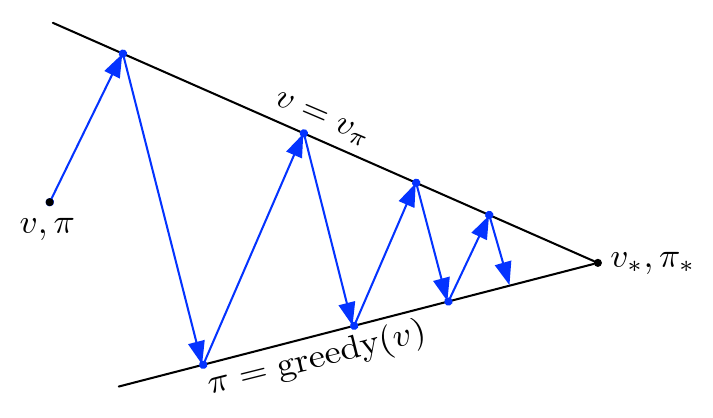
\includegraphics[scale=0.5]{GPI1.png}
    \caption{Illustration of the general policy iteration mechanism.\\Source: \citep{sutton2018}}
    \label{fig:GPI1}
    \todo[inline,color=cyan]{\textbf{To LAA:} Esta figura peguei diretamente do livro do \cite{sutton2018}, mas pretendo modificá-la ainda, evidenciando que o processo de avaliação (evalation) não precisa ser completo (a linha azul para cima não precisa ir até a preta).}
  \end{figure} 

The term \textit{generalized policy iteration} is used to designate the general ideia of letting policy evaluation an policy improvement process interact, independent of the number of steps and other details of the two process. This idea is represented in figure \ref{fig:GPI1}, where the evaluation and improvement in GPI are seen in terms of two goal, illustrated as the two black lines. The superior line represents the policy evaluation results and the inferior line, the policy improvement. Each blue line pointing to top right represents the iterations of policy evaluation before the policy improvement. The blue lines pointing to bottom right represents the policy improvement. As shown in the figure, driving toward one goal causes to move away from the other goal, e.g. making the policy greedy in respect to value function in general makes the value function incorrect for the new greedy policy and making value function evaluation typically causes the policy to be no longer greedy. But if the process continue, the processes is inevitably brought closer to the overall goal of optimality.


\section{Reinforcement Learning}
\label{sec:RL}

The basic ideas discussed about DP in previous sections can be extended to the case where no model of the system (or environment) to be controlled is unknown. This extension results in a methodology known as reinforcement learning (RL). The objective of reinforcement learning is estimate value functions and find optimal policies without the completely knowledge of the environment, as DP does. To reach this objective, RL uses actual experience, acting on the environment through an action, or the control action, and observing the imediate return, or cost.
% TODO: colocar figura aqui The figure \ref{fig:RLinteraction} exemplifies this interaction.

Two main approaches to learn the optimal policy from actual data can be defined as basis approaches to many RL algorithms.
They are the \textit{Monte Carlo (MC)} and  \textit{Temporal Difference (TD)} approaches.
Monte Carlo Methods requires only the sample sequence of states, actions and rewards from actual or simulated experience with the environment.
They uses the fact  that the value function (or cost-to-go) is the expected value of the return, expressed in \eqref{eq:cost_fun_return}. 
Using the sample sequence mentioned above, MC methods solves the RL problem based on the average sample returns in place of the true expected value, that is unknown.
The averaging sample return is updated after an episode completely occur.
% \todo[inline]{Colocar aqui o pq de nao aprofundar em MC metodos neste texto, e sim em TD.} Acho que já coloquei abaixo.
For a valid replacement of the expected value in \eqref{eq:cost_fun_return} with the sample return, the \textit{law of large numbers} needs to be applicable, i.e., a necessary condition to the sample return converges to the expected return is that the number of visits to each state $x_k$ goes to infinity. 
The problem of visit every state (or every state-action pair for control problems) is known as the \textit{exploration} problem and is inherent in RL problems and will be discussed with some more details in section \ref{sec:expandexp}.
The prediction problem (the computation of $J_\pi(\vx_k)$ and $Q_\pi(\vx_k,u_k)$), the policy improvement and the control problem (e.g.\ policy or value iterations) discussed in section~\ref{sec:DP} for DP can be adapted to be used in MC.

But, for dynamical systems control purposes, wait for an entire episode finish to update de value function and then improve policy can be a problem, mainly for real time problems.
The TD methods, solves this problem, i.e.\ updates the value function earlier, without the need of wait the entire episode to finish.
For these reason, in this thesis some TD methods will covered in detriment of the MC ones.

The next sessions presents the basis of TD methods and some extensions. 

% \subsection{Policy Iteration and Value Iteration in RL}
% \label{sec:PoVaIRL}

\subsection{The Exploration and Exploitation Dilemma}
\label{sec:expandexp}

If the policy $\pi(\vx)$ is deterministic, i.e. the actions probability matrix are composed of only 0's and 1's, following $ \pi$ will result only in the observation of the returns from one action at each state and the guarantee that every action-state pair can be visited infinite times, required for convergence of policy evaluation when using action values will not be satisfied.
% \todo{and the action and states transitions probability distributions are unknown?}
The problem of visit every action-state pair infinity times when times goes to infinity is known as the problem of \textit{maintainig exploration}. So, for problems involving action-values functions prediction, is desirable that every action is taken with a probability grater than zero, i.e., $1 > \pi(x_k) > 0$ for all $\vx_k \in \Omega_k$ to guarantee convergence in prediction. But in the opposite way, for policy improvement, is desirable that the policy be greedy, i.e. the best action in the sense that minimizes the action-value function, $Q(\vx,u)$, which results in a deterministic policy\footnote{one exception is for that cases which two or more equally valued minimum action-value function}. This is known as the \textit{exploitation problem}. This results in the \textit{exploration and exploitation dillema}.

Aiming to guarantee convergence of policy evaluation and improvement, some actions should be taken to guarantee exploration and exploitation at some degree. For RL problem, as will be treated in future sections, this dilemma can be solved with some different strategies.
One possible solution, is starting every episode, for episodic cases, in a random state, with probability grater then 1 for every state. But this solution is not feasible for continuing cases, or most dynamical control cases where the start state can not be chosen arbitrary. A most useful solution is to consider the policy as an \textit{$\epsilon$-soft} policy, where random actions are taken with $\epsilon$ probability, and deterministic actions, following the evaluated policy, are taken with probabilities  $1-\epsilon$. A common choice of  $\epsilon$-soft policy on control problems, where the policy must be improved, is use a particular  $\epsilon$-soft policy called  $\epsilon$ \textit{-greed}, where actions are chosen between a randomly one, with $\epsilon$ probability, and a \textit{greedy} policy, aiming to minimize the value function, based on evaluated policy.  
The last approach is common on what is called \textit{on-policy} control, where the policy followed by the agent are the same as the improved policy. 

Another possible solution to the exploration, exploitation dilemma is to use the \textit{off-policy} approach, where the system follows a exploratory policy, but a different policy is improved. This approach is useful for practical problems, where the system learns a better policy whiling follows a more conservative, but exploratory one. However as will see, this approach can results in convergence problems when used with value function approximation, as will see in section \eqref{sec:funcApprox}.

\subsection{Temporal-Difference Learning}
\label{sec:TDlearning}

Temporal-Difference Learning, as Monte Carlo methods, learns direct from sampled data without the need of a system model, but unlike MC methods, they don't wait for the entire episode to complete to update the estimate of the value functions $J_\pi(\vx_k)$  or  $Q_\pi(\vx_k,u_k)$, behaving, in this sense, more like DP methods. 

To reach the objective of find an optimal (or near to optimal) control policy, i.e. to solve the control problem, TD learning methods follow the pattern of the GPI where the policy is evaluated an improved, as presented in section 
% \todo{Colocar uma secao sobre GPI. Colocado: section \eqref{sec:GPI}}
\ref{sec:GPI}. 
To pursuit the optimal or quasi-optimal control, first the problem of prediction, or policy evaluation, in TD sense will be discussed. As in DP case, the policy improvement is presented in sequence, for finally, deal with some control approaches with use of TD learning.

The simplest TD method, known as \textit{one-step} TD, or \textit{TD(0)}, updates their state value function $J(x_k)$ as
\begin{equation}
  J(\vx_k) \gets J(\vx_k) + \alpha\left[r_k(\vx_k) + \gamma J(\vx_{k+1}) - J(\vx_k)\right]
\label{eq:TDupdate},
\end{equation}
% \todo{Estou com impressão que não falei sobre $\alpha$. Olhar isso. Colocado como nota de rodape.}
as long as the transition to state $x_{k+1}$ is completed and the imediate cost $r_k$ is spent.
The $\alpha$ term is a step-size parameter that, for convergence, in general needs to satisfy the standard stochastic approximation conditions\footnote
{ 
  A well-known result in stochastic approximation theory gives the conditions required to assure convergence of a sequence $\{\alpha_n(a)\}$ with probability 1:
  \begin{equation}
      \sum_{i=1}^\infty \alpha_i(a) = \infty \quad \text{and } \quad \sum_{i}^\infty \alpha_i^2(a) < \infty
    \label{eq:stochAppTeor},
  \end{equation}
  where first condition is required to guarantee that the steps are large enough to eventually
  overcome any initial conditions or random fluctuations and the second one guarantees
  that eventually the steps become small enough to assure convergence.
}.

The term $ r_k(x_k) +\gamma J(x_{k+1})$ in right hand side of \eqref{eq:TDupdate} is called the \textit{target} 
% \todo{Colocar aqui o pq to target? Comparando com outros casos? Ex. Caso MC.}
of TD method and the quantity inside the brackets measures the difference between the estimated value of $x_k$, 
% \todo{Usar um ``tilde'' em $J$ para enfatizar que é uma aproximacao?}
$J(x_k)$, and the better estimate given by the target. This difference is called the \textit{TD error} and can be defined as
\begin{equation}
  \delta_k \doteq r_k(x_k) +\gamma J(x_{k+1}) - J(x_k)
  \label{eq:TDerror}.
\end{equation}

TD error measures the estimation error \textit{made at that time} and, as it depends on the time $k+1$, it is not available until this time step is reached. A procedure for TD(0) is presented in Algorithm \ref{alg:TD0}

\begin{algorithm} % TD(0)
  \caption{Pseudo code for Policy evaluation using TD(0)}\label{alg:TD0}

  $\pi \gets $ policy to be evaluated \\
  $\alpha \gets $ value $\in \mathopen[0,1 \mathclose]$ \\
  $J(\vx) \gets$ arbitrary value $\forall \vx \in \Omega$ except for $J(terminal) = 0$

  \For{each episode}
  {
    Initialize $\vx_k$ \\
    \While{$\vx_k$ is nonterminal}
    {
      $u_k \gets$ action given by $\pi(\vx_k)$ \\
      Take control action $u_k$, observe $r_k$ and $\vx_{k+1}$ \\
      $J(\vx_k) \gets J(\vx_k) + \alpha\left[r_k(\vx_k) + \gamma J(\vx_{k+1}) - J(\vx_k)\right]$ \\
      $k = k+1$
    }
  }
  % \Return $J(x_k)$ for all $x_k \in \Omega$ \tcp*{Optimal Policy}
\end{algorithm}

\todo[inline]{Colocar mais sobre convergencia do TD(0)?} 

\subsection{On-Policy TD Control: Sarsa} 
\label{sec:sarsa}

% \subsubsection{Sarsa}
% \label{sec:sarsa}

For control purposes is desirable to learn an action-value function, or the Q-function, rather than the state-value function. The same procedure used to learn the state-value function on section \eqref{sec:TDlearning} can be used to learn the Q-function. But the state-action pair to state action pair transitions is used, instead of the state to state transitions used in TD earlier. Both the cases can be represented as Markov chains with rewards, and the same theorems assuming convergence of state values under TD(0) can be applied for action-values updates, given by
\begin{equation}
  \tqxu \gets \tqxu + \alpha\left[r_k(x_k,u_k) + \gamma \tqxuo - \tqxu\right]
\label{eq:Sarsa}.
\end{equation}
\todo[inline]{A partir daqui comecei a usar til para representar valores aproximados. Fazer isso para trás também! Para J.} 
The update of \eqref{eq:Sarsa} is done after every transition from a nonterminal state $x_k$, and $\tqxuo = 0$ if $x_k$ is terminal. This algorithm is known as 
Sarsa\footnote{The name Sarsa comes from the fact that the transitions are given as an alternate sequence of state-action-reward for stage $k$ and state-action for stage $k+1$, i.e,  $\{x_k,u_k,r_k,x_{k+1},u_{k+1}\}$, and a common notation used for states, actions and rewards on RL community is $S$,  $A$,  $R$, respectively, resulting in the sequence $\{ S_k, A_k, R_k, S_{k+1}, A_{k+1} \}$, i.e. S-A-R-S-A.} 
in RL community. The Sarsa algorithm basis is presented in the Algorithm \ref{alg:sarsa}.

\begin{algorithm} % === SARSA === Algorithm
  \caption{Pseudo code for Sarsa to estimate $\approx Q^*$ } \label{alg:sarsa}
  \DontPrintSemicolon

  $\alpha \gets  $ value $ \in  (0,1)$ \\
  $\tq(x,u) \gets$ arbitrary value $\forall \vx \in \Omega$, $u \in \mathcal{U}$, except for $\tq(terminal,\cdot) = 0$

  \For{each episode}
  {
    Initialize $\vx_k$ \\
    % Choose $u_k$ from $\vx_k$ using policy derived from $\tq$ (e.g.,  $\epsilon$-greedy)
    $u_k \gets$ action from $\vx_k$ using policy derived from $\tq$ (e.g.,  $\epsilon$-greedy) \\
    \For{step $k=0,\ 1,\ \dots, $ until the end of episode}
    {
      Take control action $u_k$, observe $r_k,\ \vx_{k+1}$ \\
      $u_{k+1} \gets$ action from $\vx_{k+1}$ using policy derived from $\tq$ (e.g.,  $\epsilon$-greedy) \\
      $\tq(\vx_k,u_k) \gets \tq(\vx_k,u_k) + \alpha\left[r_k(\vx_k,u_k) + \gamma \tq(\vx_{k+1},u_{k+1}) - \tq(\vx_k,u_k)\right]$ \\
      % $k = k+1$
    }
  }
  % \Return $J(x_k)$ for all $x_k \in \Omega$ \tcp*{Optimal Policy}
\end{algorithm}

Sarsa converges to an optimal policy as long as all state-action pairs are visited an infinite number of times. This can be accomplished using an $\epsilon-$\textit{greedy} policy, what makes the policy converge to the optimal policy with probability 1.

\subsection{Off-Policy TD Control: Q-learning} 
\label{sec:qlearning}

One of the most used off-policy methods on RL is an off-policy TD control algorithm known as \textit{Q-learning} \citep{watkins1989}, where the value function update is defined by
\begin{equation}
  \tqxu \gets \tqxu + \alpha\left[r_k(x_k,u_k) + \gamma \min_{u\in \mathcal{U}_k} \tq(x_{k+1},u) - \tqxu \right]
  \label{eq:QlearningControl},
\end{equation}
resulting in an algorithm that learns the action-value function $Q$ that directly approximates $Q^*$, i.e. the optimum action-value function independent of the policy being followed. The requirements for convergence are that all action-value state pairs are visited and updated for the policy to be improved, as required for the policy improvement theorem (Theorem \ref{teo:polImprov}) and the stochastic approximation conditions on the sequence of step-size parameters. With this conditions satisfied, $Q$ has been shown to converge with probability 1 to  $Q^*$ for the tabular case \eqref{eq:QlearningControl}. The Algorithm \ref{alg:Qlearning} shows a procedure to Q-learning.

\begin{algorithm} % [Q-learning]
  \caption{Pseudo code for Sarsa to estimate $\tq \approx Q^*$ }\label{alg:Qlearning}
  \DontPrintSemicolon

  $\alpha \gets $ value $\in (0,1]$ \\
  $\tq(x,u) \gets$ arbitrary value $\forall \vx \in \Omega,\ u \in \mathcal{U}$, except for $\tq(terminal,\ \cdot\ ) = 0$

  \For{each episode}
  {
    Initialize $\vx_k$ \\
    % Choose $u_k$ from $\vx_k$ using policy derived from $\tq$ (e.g.,  $\epsilon$-greedy)
    \For{step $k=0,\ 1,\ \dots, $ until the end of episode}
    {
      $u_{k} \gets$ action from $\vx_k$ using policy derived from $\tq$ (e.g.,  $\epsilon$-greedy) \\
      Take control action $u_k$, observe $r_k,\ \vx_{k+1}$ \\
      $\tq(\vx_k,u_k) \gets \tq(\vx_k,u_k) + \alpha\left[r_k(\vx_k,u_k) + \gamma \min_{u \in \mathcal{U}_k} \tq(\vx_{k+1},u_{k+1}) - \tq(\vx_k,u_k)\right]$ \\
      % $k = k+1$
    }
  }
  % \Return $J(x_k)$ for all $x_k \in \Omega$ \tcp*{Optimal Policy}
\end{algorithm}

% TODO: Colocar as seguintes seções?
% \subsubsection{Q-learning}
%   \label{sec:qlearning}
% \section{$n$-step Bootstrapping?}%
%   \label{sec:n_step_bootstrapping}


\section{Function Approximation}
  \label{sec:funcApprox}

Until now, the value functions $J(\vx)$ and  $Q(\vx)$ was considered as a lookup table, i.e. the states was considered as \todo{não estou certo se a palavra seria \textit{discretizada} mesmo. Quantizada, talvez?} discrete and finite values in state space. In the same form, actions are considered as discrete values too. The tabular approach is useful for discrete in state-action systems, where the number of state-action pairs are relatively small. For systems with huge state-action pairs or where states are treated as continuous values, resulting in continuous a new approach is needed. To aim this objective, the concept of function approximation is introduced in this and next sections. First, in this section this approximation is done by what will be called value-function approximation. In this methodology, the value-functions (state-value and action-value) are approximated with continuous functions as described in sequence.
This type of approximation, make possible to represents continuous states and their related value functions, but they do not deal with continuous action spaces. To deal with continuous action spaces, policy gradient method are presented at the end of the section.

% a parameterized functional form, with parameters represented as a vector $\vpfa \in \R^d$, where $d$ is the number of parameters. This parametric approximation will be represented by $\Jfa_\pi(\vx,\vpfa)\approx J_\pi(\vx)$ for a policy $\pi$.

\subsection{Value-Function Approximation}
  \label{sec:valFunApp}

The methods discussed so far, all updates an estimated value function of a state toward an better prediction that includes the most recent data collected.
From now on, that better prediction will be called \textit{update target}.
The notation $x \mapsto T$, where $x$ is the state where the value function was updated an $T$ is the \textit{update target}, will be used.
This update indicates that the estimated value of $x$ should be more like the updated target  $T$.
For example, with this notation, the TD(0) update can be written as $x_k \mapsto r_k + \gamma \Jfa(\vx_{k+1},\vpfa_k)$\footnote
{
  here the parametric approximation $\Jfa(\vx,\vpfa_k)$ is used in place of the value function estimative $\hat{J} (\vx_k)$ of tabular method presented in Section~\ref{sec:TDlearning}.
}.
The update target represents the old value estimation updated with the most recent information (e.g., the imediate cost $r_k$ on TD(0) presented above).
\todo{Acho que faltou ``apresentar'' o vetor de parametros $\vpfa = \begin{bmatrix} \pfa_1 & \pfa_2 & \cdots & \pfa_d \end{bmatrix}^T $} 
A wide range of function approximation methods have been studied in scientific community, on last decades. This methods aim to reproduce the same input-output relation of a collected data.
Many of this existing methods of function approximations, some better then others, can be used for value  predictions on RL, using the $x \mapsto T$ of each update as a training example.
This value function predictions is used as an estimated value function.
For RL purposes, methods that can learn online and that are able to handle with nonstationary target functions are, in general, required.
Most of the function approximation methods are parametric, in the sense that they seeks for a parametric function that approximates of the true value function by adjusting the parameters until some objective is archived.
As in this thesis we deal only with parametric methods, only this class of functions approximations will be studied.
Besides the parametric or nonparametric classes, function approximation methods can be classified as \textit{linear methods} and the \textit{nonlinear methods}.
In booth of this classes, the objective is to find a parametric function that approximates the value functions for, in general, huge state spaces, continuous or not, that makes difficult or impossible to be treated as a lookup table.
Basically, the difference between this two linear and nonlinear methods are that, in the former, the functions are linear in the parameters, and in the last, not.
In the next sections some of this methods are briefly presented, starting with the linear ones that, as will discussed later, in general, presents more convergence guarantees.

When using function approximation there is far more states than parameters, so an update at one state affects many others and is not possible to get the values all exactly correct.
To deal with it, is common to specify a state distribution $\mu(\vx) \ge 0,\ \sum_\vx = 1$, representing how much the error in each state are valuable.
So the difference between the approximate values $\Jfaxp$ and the true value  $J_\pi(\vx)$ is defined as the \textit{Mean Squared Value Error}, denoted here with $\overline{VE}$, and expressed as
\begin{equation}
  \overline{VE}(\pfa) \doteq \sum_{\vx \in \Omega} \mu(\vx) {\left[ J_\pi(\vx) - \Jfaxp \right]}^2
  \label{eq:VE}.
\end{equation}
The distribution $\mu(\vx)$ is called  \textit{on-policy distribution} and is commonly taken to be the fraction of time to be spent in $\vx$.

As mentioned earlier, there is a wide range of function approximation methods that can be used in reinforcement learning.
Here the methods based on gradient principles, like linear gradient descent methods will be explored, once they are used in this work.
In next sections, a brief about stochastic-gradient and semi-gradient methods is presented.
In sequence, some basics off function approximation for linear and non linear methods are presented as well. 

\subsection{Stochastic-gradient Methods}%
  \label{sub:stochastic_gradient_methods}

Stochastic-gradient descent (SGD, for short) methods are the most used of all approximation methods well suited for reinforcement learning.
In this methods, the approximate value function $\Jfaxp$ is a differentiable function of the parameter vector  $\vpfa$ for all  $\vx \in \Omega$. 

Assuming that the states are sampled (one at a time or in a batch way), the goal is to minimize the $\overline{VE}$, given in \eqref{eq:VE}, trying to minimize the error over the observed samples.
To do that, SGD methods adjust the parameter vector $\vpfa$ after each sample by a small amount in the direction which the error are most reduced, what can be expressed as
 \begin{align}
   \vpfa_{k+1} &\doteq \vpfa_k -\frac{1}{2}\alpha\nabla\left[J_\pi(x_k)-\Jfaxpk\right]^2 \label{eq:SGD_1}\\
            &= \omega_k + \alpha \left[J_\pi(x_k) - \Jfaxpk\right]\nabla\Jfaxpk
   \label{eq:SGD_2},
\end{align}
where $\alpha > 0$ is a step size parameter and $\nabla f(\vpfa)$, represents the gradient of any scalar function $f(\vpfa)$, expressed as a column vector given by
 \begin{equation}
  \nabla f(\vpfa) \doteq \left(\frac{\partial f(\vpfa)}{\partial\pfa_1},\ \frac{\partial f(\vpfa)}{\partial\pfa_2},\ \dots,\ \frac{\partial f(\vpfa)}{\partial\pfa_d} \right)^T
  \label{eq:grad}.
\end{equation}
So, SGD is a gradient descent method because they take a step in $\vpfa_k$ proportional to the negative gradient of the sampled squared error \eqref{eq:SGD_1}, and stochastic because the update is done in only a single sample, which might have been selected stochastically.
Over many samples, the overall effect is to minimize an average performance measure, like $\overline{VE}$ \eqref{eq:VE}.

The convergence to, at least, a local minimum of the performance measure, is guaranteed if $\alpha$ decreases over time in such a way that the  \textit{standard stochastic approximation conditions} (see footnote in section \eqref{sec:TDlearning}) are satisfied.

In \eqref{eq:SGD_1} and \eqref{eq:SGD_2}, the true state-value function $J_\pi(\vx)$ was used.
But this value is unknown on RL methods and the target $T_k$ is used in place of  $J_\pi(\vx)$, yielding in the following general SGD method 

\begin{equation}
\vpfa_k \doteq \omega_k + \alpha \left[T_k - \Jfaxpk\right]\nabla\Jfaxpk
\label{eq:genSGD}.
\end{equation}
Again, the convergence guarantees are satisfied under stochastic approximation conditions for a decreasing $\alpha$, but only if $Tkk$ is an  \textit{unbiased} estimate, i.e. $ \mathbb{E}[T_k|\vx_k=\vx] = J_\pi(\vx_k)$.
This is the case for Monte Carlo RL methods, but isn't the case for TD RL methods.

In TD RL methods, the target $T_k$ depends on the current value of the parameter vector  $\vpfa_k$, which results in a biased estimation and do not produces a true gradient-descent method.
The step from  \eqref{eq:SGD_1} to \eqref{eq:SGD_2} isn't valid in this case, because it relies on the independence of the target on $\vpfa_k$.

So, TD RL stochastic gradiente methods, or other methods that relies on 
% \todo{colocar significado de bootstraping aqui? Acho que não coloquei ainda. Checar.}
bootstrapping\footnote{bootstrapping methods are methods where bases they update in part on an existing estimate.}, that uses the update \eqref{eq:genSGD} are called \textit{stochastic semi-gradient methods}.

% TODO: Bootstrapping Update targets that include existing estimates (as in dynamic programming or TD methods) rather than relying exclusively on actual rewards and complete returns (as in MC methods).

Although semi-gradient methods do not converge as robust as the gradient methods, it converges reliably in linear case presented on next section.
Furthermore they results in faster learning and enables the learn to be continual and online without waiting for the end of the episode, which is good for continuing problems.
\todo[inline]{Colocar algoritmo para o TD(0) aqui? Acho que vou deixar para o caso do controle (SARSA, ou algo do tipo). Está ficando com muito algoritmo.}  


\subsection{Linear Function Approximation Methods}%
\label{sub:linear_function_approximation_methods}

Linear function approximation methods aim to approximate the state value function $J(\vx)$, for the prediction problem, or the action value function  $Q(\vx,u)$, for control problem, as parametric functions $\Jfa(\vx,\vpfa)$, or  $\Qfa(\vx,u,\vpfa)$, respectively. This approximation is done by means of the correct choice of the vector parameter $\vpfa$ that satisfies some criteria. The advantage is that, with a relative small size parameter vector $\vpfa \in \R^d$ and a same size real-valued vector $\vv(\vx) = \begin{bmatrix} x_1 & x_2 & \dots & x_d \end{bmatrix}^T $, the approximate value function can approximate the actual value function, for any real value of the state $\vx$. The vector $\vv(\vx)$ is called a \textit{feature vector} representing state $\vx$, with  $\vv_i(\vx) : \Omega \mapsto \R$ for each component $\vv_i(\vx)$. The state-value function are related with this vectors by the approximation
\begin{equation}
  \Jfaxp \doteq \vpfa^T \vv(\vx) \doteq \sum_{i=1}^d \pfa_i v_i(\vx)
  \label{eq:state-value-fa},
\end{equation}
where $\pfa_i$ and $v_i(\vx)$ are the parameter $i$ and the feature $i$, respectively, with  $i = 1,\ 2,\ \dots,\ d$.

For linear methods, the features form a linear basis for the set of approximate function, what make them basis functions. 
% \todo{Colocar aqui alguns dos possíveis métodos com referencias} Coloquei alguns parágrafos para a frente.
The diferente ways that features can be defined is what results in diferente methods of linear function approximations, as we see in next sections. But all of them share some basic properties, as will be presented in this section.

When using SGD updates with linear function approximation, the update \eqref{eq:genSGD} results in a particular simple for given as
\begin{equation}
  \vpfa_k \doteq \omega_k + \alpha \left[T_k - \Jfaxpk\right]\vv(\vx_k)
  \label{eq:lingenSGD},
\end{equation}
since the gradient $\nabla \Jfaxp = \vv(\vx)$ for a linear in parameter function.

One advantage of linear methods is that there is only one optimum (or a set of equals optimums for degenerated cases), and any method that guarantees the convergence to (or near to) a local optimum guarantees the convergence to (or near to) the global optimum.

The TD(0) using SGD linear function approximation, which is, in fact, a semi-gradient descent method, as discussed above, can be proved to converge the parameter vector to a point near of the global optimum \todo{Colocar esta prova? Talvez como anexo. A principio acho que não convém.}  \citep{sutton1988}, which is known as \todo{colocar o desenvolvimento do pq converge para um ``TD fixed point''?} \textit{TD fixed point}, and results, for the continuing case, in a $ \overline{VE}$ bounded as
\begin{equation}
  \overline{VE}(\vpfa_{TD}) \le \frac{1}{1-\gamma} \min_{\vpfa}\overline{VE}(\vpfa)
  \label{eq:meanSquaredValueError}. 
\end{equation}
This kind of convergence and bounds on $\overline{VE}$ applies to other on-policy bootstrapping methods as well. \citet{bertsekas1996} proved an analogous bound for the episodic case as well.
% Nevertheless, this convergences, is proved to linear function approximation using SGD updates for some on-policy bootstrapping (semi-gradient) methods with on-policy distribution. For off-policy cas

As stated before, the diferente ways that features can be defined results in diferente methods of linear function approximations, like \textit{Polynomials}, \textit{Fourier Basis} \citep{konidaris2011}, \textit{Coarse Coding} \citep{hinton1984,waltz1965}, \textit{Tile Coding} \citep{albus1971,watkins1989}, \textit{Radial Basis Functions} \citep{powell1987}, among others.

% Konidaris, Osentoski, and Thomas (2011) -> Fourier basis in a simple form suitable to reinforcement learning (with multidimentional continuous state spaces and functions that do not have to be periodic.
% Coarse coding -> Hinton (1984). Waltz and Fu (1965) example of this type of FA in RL
% Tile coding -> Albus(1971, 1981) -> introduced. Miller and Glanz (1996) -> deal with it.
% Radial Basis: Powell (1987), Broomhead and Lowe (1988), Poggio and Girosi (1989, 1990).

Here, in this work, only a brief introduction to polynomial and radial basis functions are given, since they are more relevant to this work. An introduction to another linear function approximations can be found on \citet{sutton2018}. In next sections this two methods are presented.

\subsubsection{Polynomials features for Function Approximations}
\label{sec:polynomial}

Polynomials are maybe, the most intuitive way to represents features for linear methods. This fratures representation are possible when problems can be expressed as numbers. Polynomials belongs to a family of features used for interpolation and regression, and might be the easiest way to introduce the concept of features construction.

Polynomials can be used to represent linear system, for example, a second order linear system, (such as model of a moving cart), could be represented with a two dimensional features vector $\vv(\vx) = \begin{bmatrix} v_1 & v_2 \end{bmatrix}^T $, with $ v_1 = x_1$ and $ v_2=x_2$, where $ x_1$ represents the first state variable and $ x_2$ (such as the cart position), the second (such as the cart velocity).

The example above shows the idea of a linear system representation with polynomials, but they could be used to represent nonlinear systems as well, since it continues to be linear in parameters. It enables for example, take into account interaction between the two states, or representation of affine functions in the original state numbers. For example, for a system with two states the feature $\vv_{\vx} = \begin{bmatrix} 1 & x_1 & x_2 & x_1x_2 \end{bmatrix}^T$ could be chosen, where $ x_1x_2$ represents the interaction and the term 1 allow the representation of the afine functions. More complexes features could be chosen as well, like one including terms like $ x_1^2$, $ x_2^2$, as well.

The general case can be state as follows.
Suppose a state vector $\vx \in \R^n$. For this $n$-dimensional state space, each polynomial basis of order  $k$ can be written as
 \begin{equation}
   v_i(\vx) = \prod_{j=1}^{n}x_j^{c_{i,j}} ,
\end{equation}
where each $c_{i,j}$ is an integer in the set $[0,k]$ for $n\ge 0$. This results in a order-$n$ polynomial basis for dimension $n$, and in  $(k+1)^{n}$ features.

In general, higher-order polynomials results in more accurate approximations, but features of order $k$ basis grows exponentially with the state space dimension $n$ (for $k>0$). In practice, generally, a subset the features are chosen based on some criteria, like prior beliefs about the nature of the system or some existent methods for polynomial regression.

\subsection{Nonlinear Function Approximations}
\todo[inline,color=cyan]{Saltei esta seção pois não sei se usarei (e por prioridades). Mas bem provável que sim. O foco aqui seria falar sobre aproximação por redes neurais, principalmente.} 
\subsection{On-Pollicy Control with function approximation}
\subsection{Off-Policy Control with function approximation}
\label{sec:offPoliceControlFA}




\subsection{Policy Gradient Methods}
\label{sec:PGM}


Policy gradient methods are function approximation methods as value-function approximation methods addressed on previous sections. However, instead of learn the values of actions an then select actions based on their estimated values, policy gradient methods learn a \textit{parametrized policy} directly. This allows to select actions without the use of a value function.

In policy gradient approach, the policy will be a parametrized function $\pi(u|\vx,\vt) =$ $\text{Pr}\left\{u_k=u | x_k = x, \vt_k = \vt\right\}$, i.e. the probability of taken the action $u$ at stage $k$. Where $\vt \in \R^{r}$ is the policy parameter vector, with $r = |\mathcal{U}|$.

The objective is to learn the policy parameter vector $\vt$ that minimizes some performance measure $P(\vt)$. It is done by updating the parameter vector in the direction whre the performance measure most decreases, i.e.
according to the gradient descent approach given by 
% To learn the policy parameter, these methods use the gradient of some performance measure $P(\vt)$, function of the parameter $\vt$ to update the parameter accoding to a gradient descent approach to minimize\footnote{sometimes is required to maximize the performance measure.l, resulting in a \textit{gradient ascent} $\vt_{k+1} = \vt_k + \alpha \apPG$.} the performance, the parameters are updated according to a gradient descent in $P(\vt)$:

\begin{equation}
\vt_{k+1} = \vt - \alpha \apPG
\label{eq:PGpar},
\end{equation}
where $\apPG \in \R^r$ is a stochastic estimate whose expectation approximates the gradient of the performance measure with respect to $\vt_k$.

Policy gradient methods can handle feasible discrete action spaces (where the action space is not too large an can be implemented in practice, as a lookup table), as huge  (where the number of actions are so large that tabular methods become impracticable) or continuous ones (with infinite number of actions).

If the action space is small enough a natural to define the policy as a numerical lookup table function $h(\vx,u\vt) \in \R$ for each state-action pair, commonly called as \textit{preferences}.
The idea is that the actions with highest preferences in each state presents higher probabilities to be selected. 
One example is an exponential distribution parametrization known \textit{soft-max in action preferences}, where
\begin{equation}
  \pi(u|\vx,\vt) = \frac{\exp{\left(h(\vx,u,\vt)\right)}}{\sum_{b \in \mathcal{U}} \exp{\left(h(\vx,b,\vt)\right)}}
\label{eq:softmax}.
\end{equation}
The actions preferences can be parametrized arbitrary, as a neural network, or linear in feature, or another method described in section \eqref{sec:funcApprox}.
If linear in features the preferences is written as
\begin{equation}
  h(\vx,u,\vt) = \vt^T\vv(\vx,u),
\end{equation}
using features vectors $\vv(\vx,u) \in \R^r$ constructed with one of the methods cited at end of section \eqref{sub:linear_function_approximation_methods}.

The main advantages of this kind of policy parametrization is that it enables to find stochastic optimal policies (whereas action-value methods can't do naturally), but can be used to approach a deterministic policy as well, where the actions are selected in an $\epsilon$-greedy manner.

\todo[inline,color=cyan]{ Falta coisas aqui ainda. Na verdade acho que essa abordagem usando Policy Gradient Methods deve acabar sendo mais útil para mim.}

% \begin{equation}
% \vt^T\vv(\vx,u), .
% \end{equation}

\subsubsection{Parametrization for continuous actions}

To deal with huge or continuous action spaces the general procedure is the same as the tabular case, but now, instead of learn the probabilities for each of the actions, the procedure look to learns the statistics of the probability distribution.

One common choice is to parametrize the policy as the normal probability density aver a real-valued scalar action, with standard deviation $\sigma(\vx,\vt)$ and mean $\mu(\vx,\vt)$ given by the following parametric function approximation:
\begin{equation}
  \pi(u|\vx,\vt) \doteq \frac{1}{\sigma(\vx,\vt)\sqrt{2\pi} } \exp{\left(-\frac{(u-\mu(\vx,\vt))^2}{2\sigma(\vx,\vt)^2}\right)} ,
\end{equation}
where the standard deviation and the mean is defined as a parametric function of $\vt$. For example, they can be defined as
 \begin{equation}
 \sigma(\vx,\vt) \doteq \exp{\left(\vt_\sigma^T\vv_\sigma(\vx)\right)} \quad \quad \text{and }
   \quad \mu(\vx,\vt) \doteq \vt_\mu^T\vv_\mu(\vx) ,
\end{equation}
with $\vt= \begin{bmatrix} \vt_\sigma & \vt_\mu \end{bmatrix}^T$,  $\vv_\sigma$ and $\vv_\mu$ representing a state feature vector that could be constructed using some method as cited on section \eqref{sec:funcApprox}.
Note that the standard deviation is a always positive value, for this reason is defined as an exponential function.


% \section{Infinite Horizon Problems}
% \label{sec:IHP}
%
% Since for dynamic control problems the trajectory of the system to be controlled is, in most of the cases, given in a infinite-step way, here we will try to deal with this case with more details. \todo[size=\tiny]{Talvez colocar isso na introdução do capítulo, falando que o objetivo do capítulo é chegar nesse ponto, mas para isso alguns conceitos fundamentais (casos mais simples?) devem ser tratado antes.}
%
% The main difference between the infinite horizon and the finite horizon RL problems, despite the obvious fact that in the former the number of stages are infinite, is that the system is stationary. It means that the state equation, the stage cost and the probability distribution of the random disturbance do not change from one to stage to the next \citep{bertsekasReinforcementLearningOptimal2019}.
%
% The stationarity assumption can be a problem to some practical time variant dynamical systems, but for many cases where the system parameters vary slowly with time, this assumption gives a good approximation.
%
% Infinity horizon problems, in general, results in simpler optimal policies than the finite case, which often presents a stationary behavior. But in the other hand the mathematical treatment can be more complex.
%
% The total cost of a policy $\vpi = {\mu_0, \mu_1, \dots}$ for a infinite horizon stochastic problem is given by
%
% \begin{equation}
  % J_\pi(\vx_0) = \lim_{N \to \infty} \E_{\vw_k} \left\{ \sum_{k=0}^{N-1} \gamma^{k} r(\vx_k,\vmu_k(\vx_k),\vw_k) \right\}
% \label{eq:JIH}.
% \end{equation}
% The term $\gamma$ is a positive scalar, and $\gamma <1$ results in a discount factor meaning that the present cost is more important than the future ones; and $\E_{\vw_k}$ means the expected value over all random disturbances  $\vw_k$, with $k = 0, 1, \dots$, until infinity. For now, the limit in \eqref{eq:JIH} is assumed to exists.
% In a procedure like that shown in sections \ref{sec:VaIDP} and \ref{sec:VaIRL}, the optimal cost-to-go function $J_N$ corresponding to $N$-stages finite horizon problem can be written according to the Value Iteration Algorithm that follows \todo{Tem coisas erradas aqui! 1- é $J_N$ mesmo? Não seria $J^*$? Acho que $J^*_N$ 2- a eq.  \eqref{eq:VIalgorithm} não é o caso ótimo!}
%
% \begin{equation}
  % J_{k+1}(x) = \min_{u\in \mathcal{U}} \E_{\vw_k} \left\{ r(\vx,\vu,\vw) + J_k\left(f(\vx,\vu,\vw)\right) \right\}, \qquad k = 0, 1, \dots, N-1
% \label{eq:VIalgorithm},
% \end{equation}
% starting from the initial condition $J_0(x)=0$, $\forall x$.
%
% The optimal infinite horizon can be expressed as
% \begin{equation}
  % J^*(x) = \lim_{N \to \infty}J_N^*(x)
% \label{eq:OptInfHOriz}.
% \end{equation}
%
% Minimization of \eqref{eq:JIH} can be accomplished with two strategies, denominated as
% \begin{itemize}
  % \item Stochastic shortest path problems (SSP)
  % \item Discounted problems.
% \end{itemize}
%
% % The next sections presents these to strategies.
% The next sections gives an introduction on these to strategies.
%
% \subsection{Stochastic Shortest Path}
%
% In Stochastic Shortest Path (SSP), is assumed that there is no discount factor, i.e. $\gamma = 1$ in~\eqref{eq:JIH} and there is a \emph{special terminal state t with cost free}, i.e.\ when the trajectory reaches that state, it remains there with no future cost. It can be formally written as
% \begin{equation}
  % p_{tt}(\vu) = 1, \quad r(t, \vu, t) = 0, \qquad \forall \ \vu \in \mathcal{U}
% \label{eq:SSP_1}.
% \end{equation}
% where \todo{colocar sobre essa probabilidade na seção~\ref{sec:SDP}?} $p_{ij}(\vu)$ means the probability of, at state $i$, taking a control action $\vu$, the system trajectory is driven to state $j$; and $r(i,\vu,j)$ represents the cost of the transition from state $i$ to  $j$ when control action $\vu$ is taken.
%
    % \begin{figure}[htpb]
        % \centering
        % % \includegraphics[width=0.8\textwidth]{}
        %     \begin{tikzpicture}[->,>=stealth',shorten >=1pt,auto,node distance=3cm, thick]
      \tikzstyle{every state}=[draw=black,fill=blue!20,text=black]
      % \tikzstyle{dots}=[thick,draw=none,fill=none,text=black]
      % \tikzstyle{place}=[draw=none,fill=none,text=black!75]
      % \tikzstyle{texto}=[draw=none,fill=none,text=black]
      \node[state] (i) {$i$};
      \node[state] (j) [right of=i] {$j$};
      \node[state] (t) [above of=i,xshift=1.5cm,yshift=-0.8cm] {$t$};

      \path[->]
          (i) edge [loop left] node {$p_{ii}(\vu)$} ( )
          (j) edge [loop right] node {$p_{jj}(\vu)$} ( )
          (t) edge [loop above] node {$p_{tt}(\vu) = 1$} ( )
          (i) edge [bend left] node {$p_{ij}(\vu)$} (j)
          (j) edge [bend left] node {$p_{ji}(\vu)$} (i)
          (i) edge node [left] {$p_{it}(\vu)$} (t)
          (j) edge node [right] {$p_{jt}(\vu)$} (t);
          % (C) edge node {c} (D);
    \end{tikzpicture}

        % \caption{Transition graph representing a MDP of a minimum SSP problem.}
        % \label{fig:stages}
      % \end{figure} \todo[inline]{Terminar. Melhorar caption. \st{Mexer na altura?} Contextualizar.}
%
